\begin{figure*}[p]
	\centering
	\begin{subfigure}[t]{\columnwidth}
		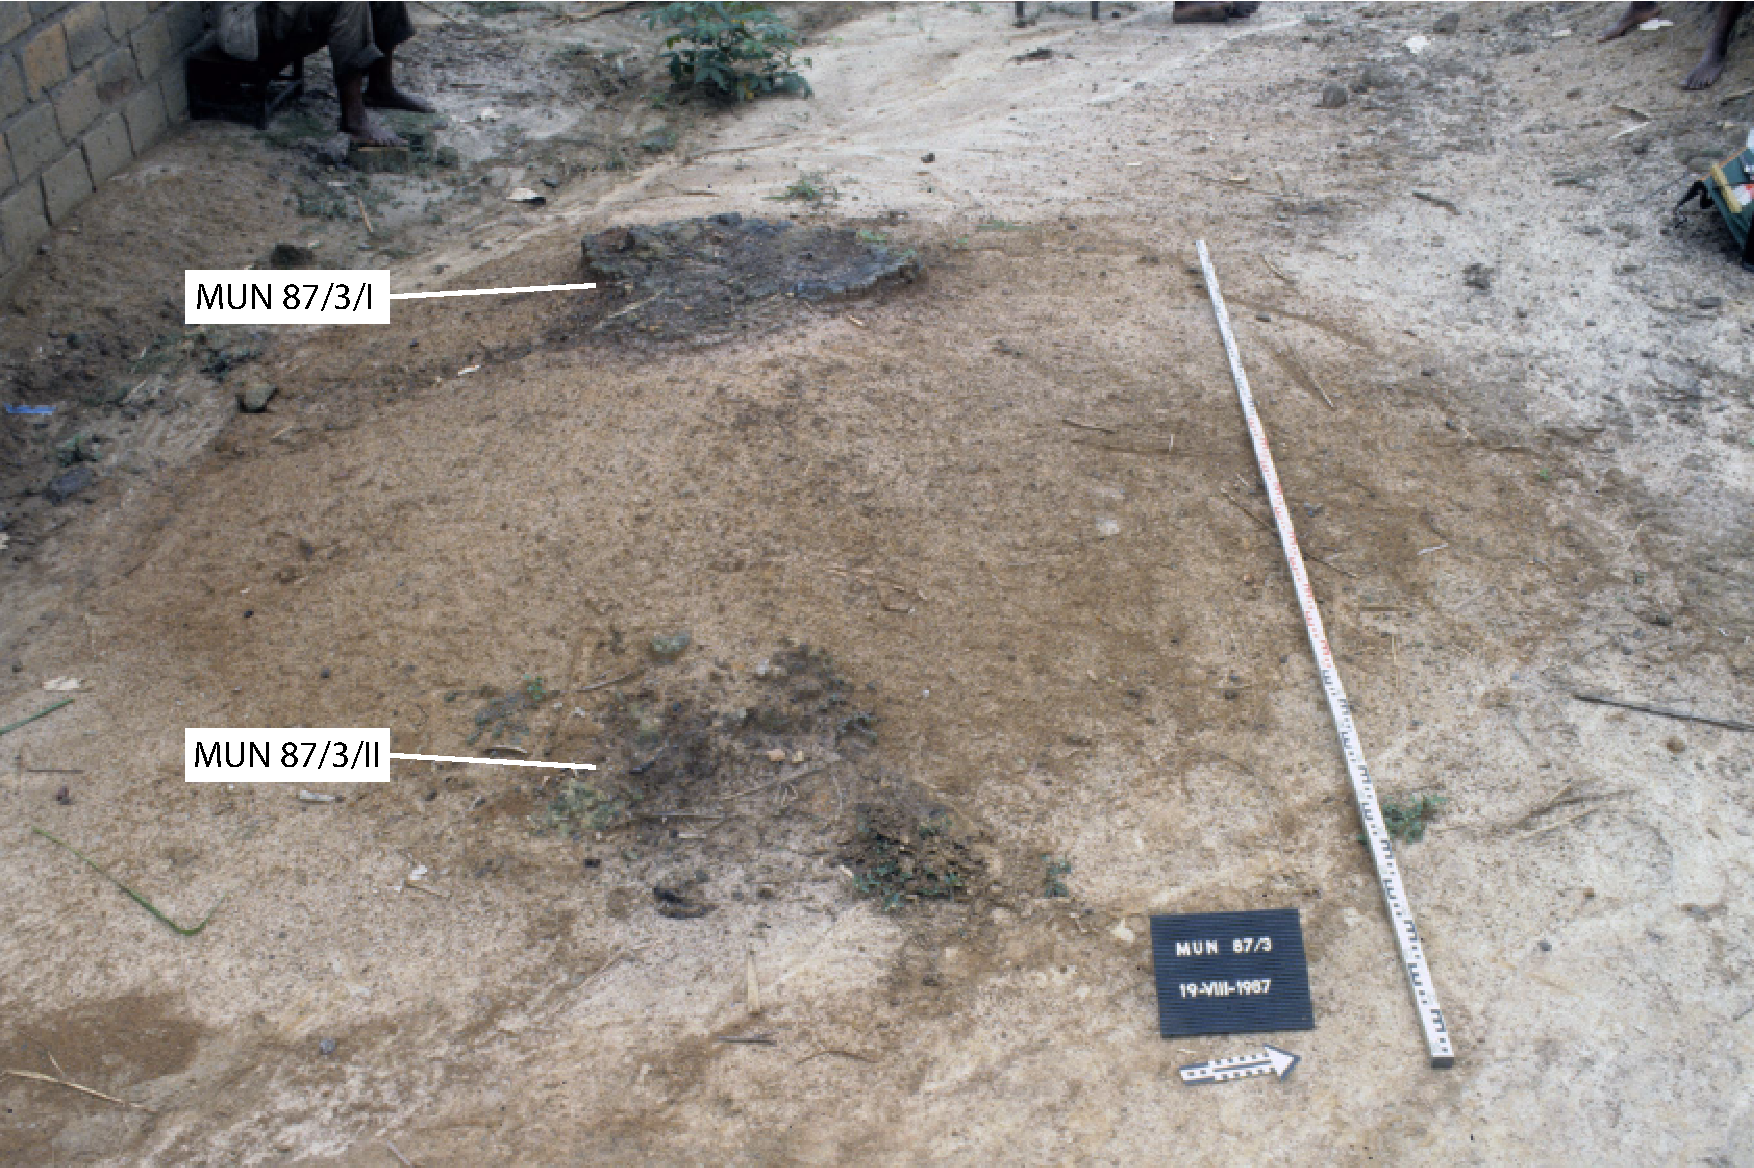
\includegraphics[width=\textwidth]{fig/MUN87-30_H87-03-18-01.pdf}
		\caption{MUN~87/3: Ansicht von Westen (Foto: H. Holsten, 1987).}
		\label{fig:MUN87.3-0_Foto}
	\end{subfigure}\hfill
	\begin{subfigure}[t]{\columnwidth}
		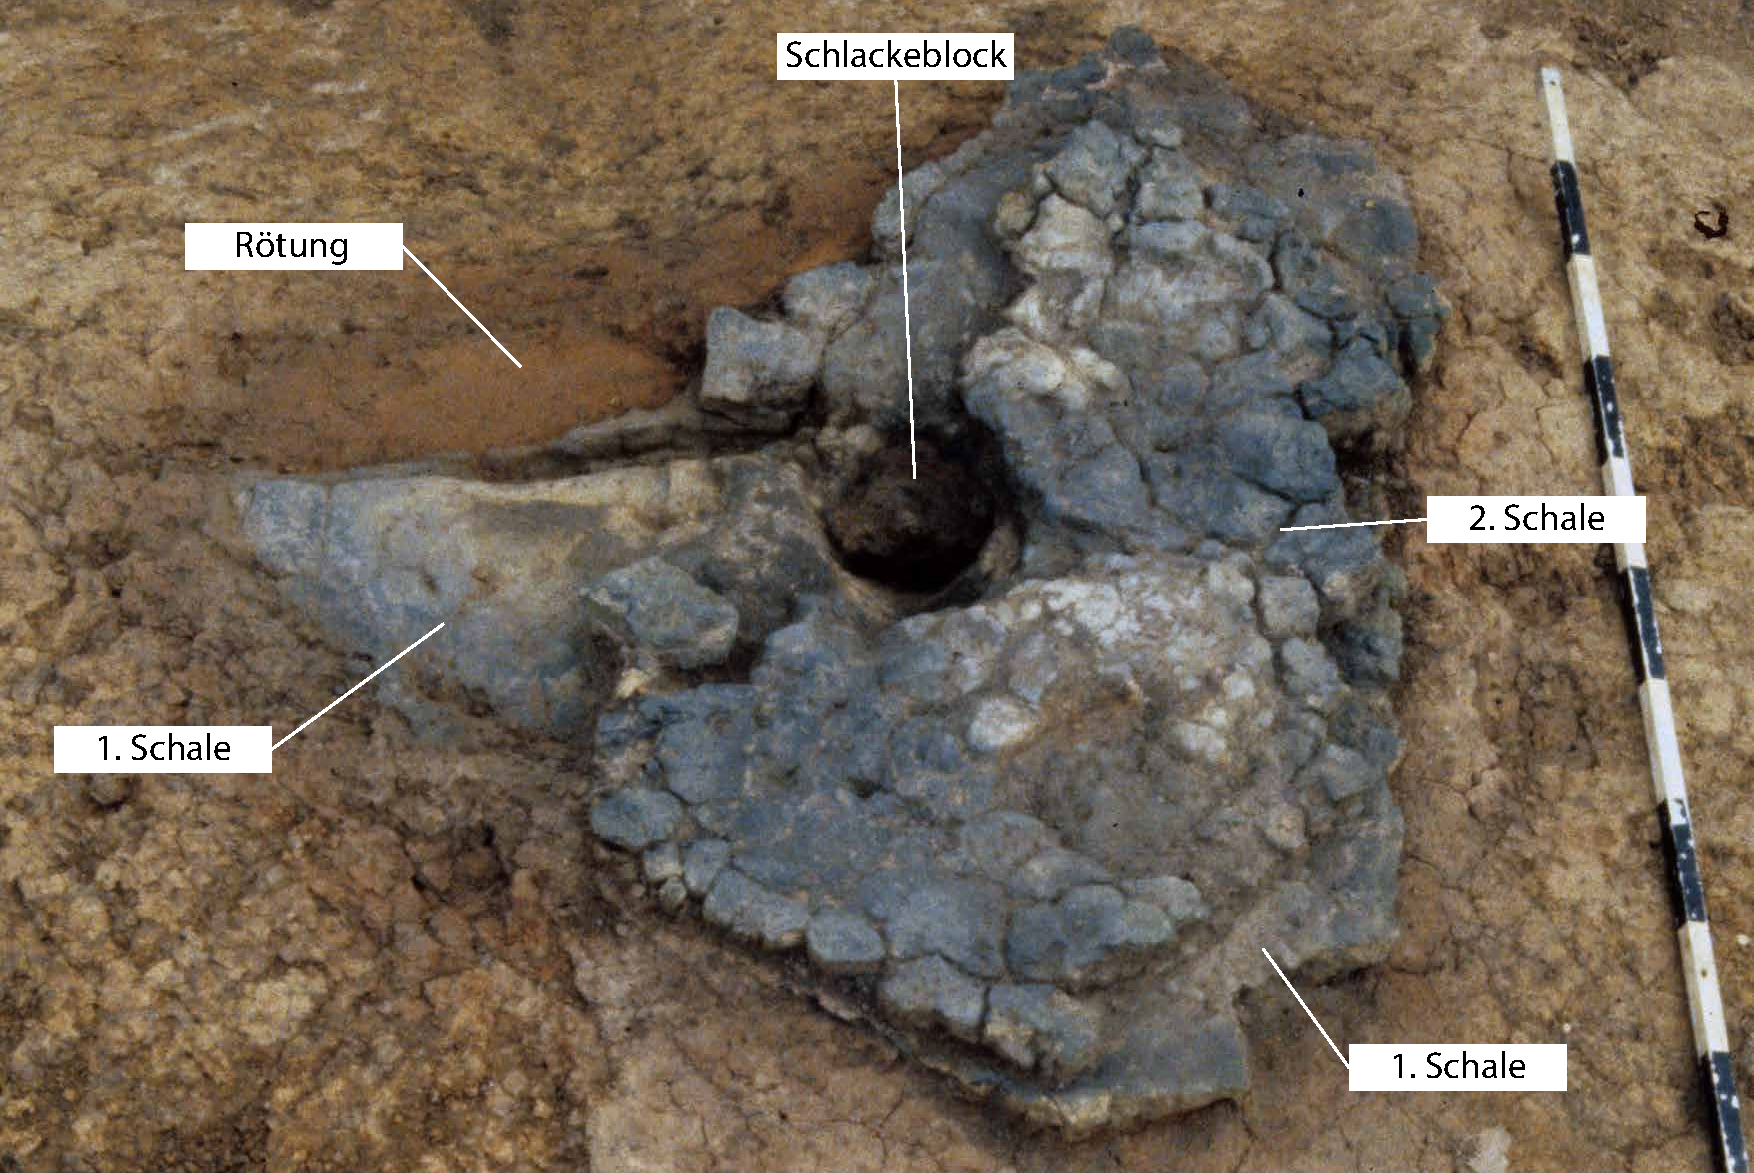
\includegraphics[width=\textwidth]{fig/MUN87-3-I_E-87-038-34_kompr.pdf}
		\caption{MUN~87/3/I: Aufsicht auf die Ofenplattform (Foto: M. K. H. Eggert, 1987).}
		\label{fig:MUN87-3_Planum}
	\end{subfigure}
	\begin{subfigure}[t]{\columnwidth}
		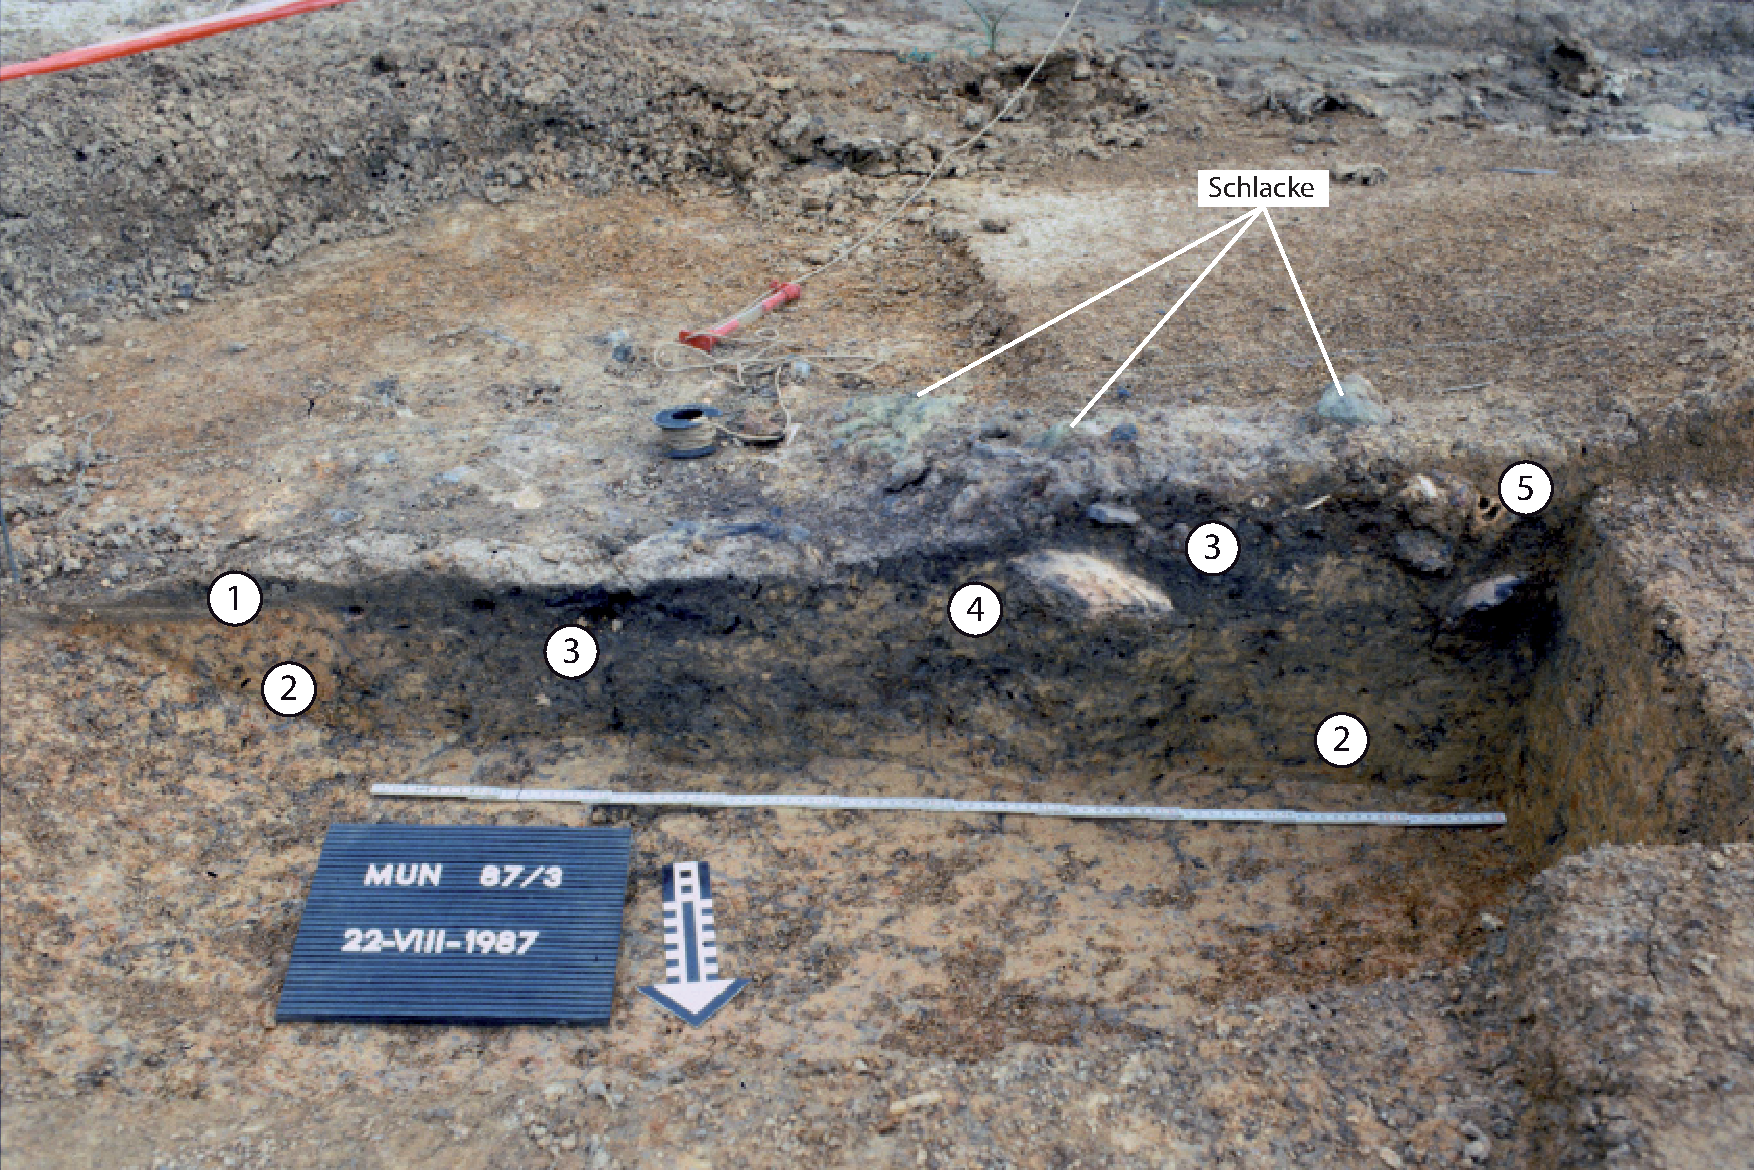
\includegraphics[width=\textwidth]{fig/MUN87-3-II-4_H87-04-37.pdf}
		\caption{MUN~87/3/II: Profil durch die Keramik-Schlacke-Konzentration (Foto: H. Holsten, 1987).}
		\label{fig:MUN87.3.II-3_Foto}
	\end{subfigure}\hfill
	\begin{subfigure}[t]{\columnwidth}
		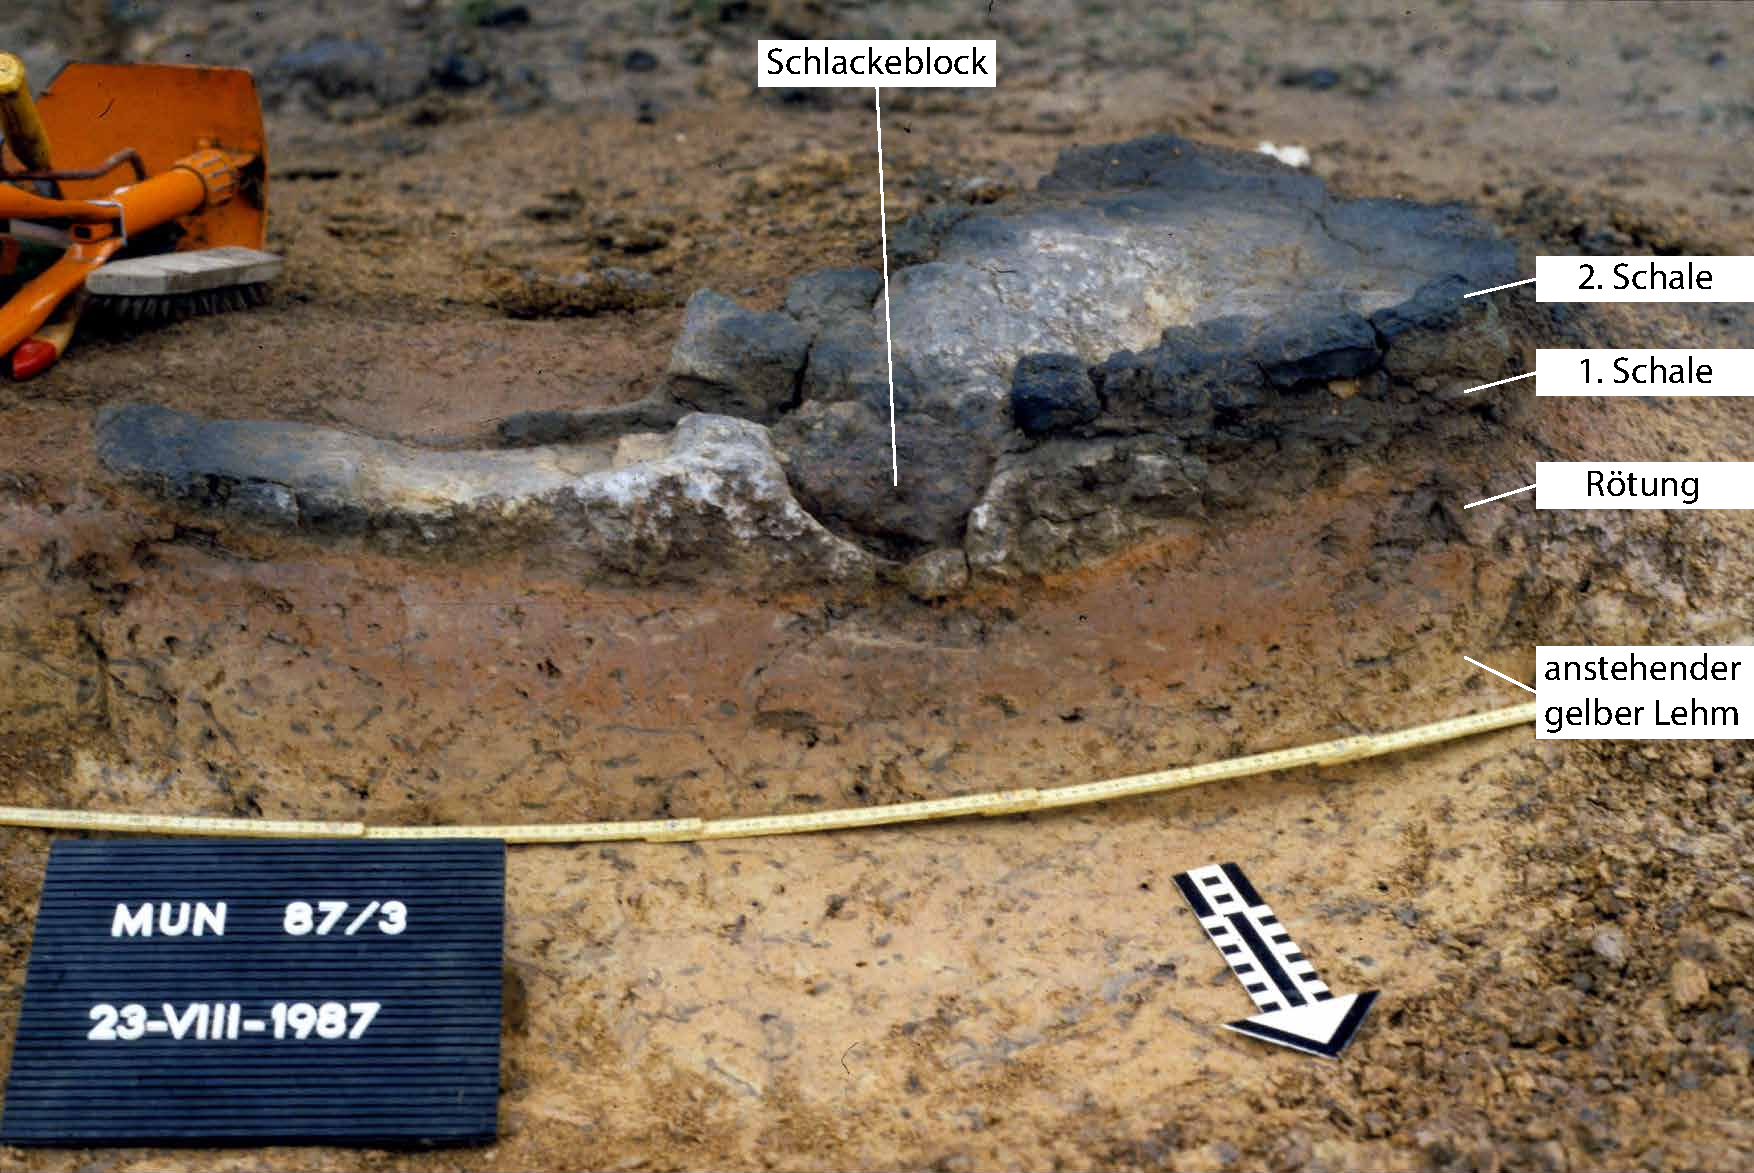
\includegraphics[width=\textwidth]{fig/MUN87-3-I_H-87-05-9_kompr.pdf}
		\caption{MUN~87/3/I: Südprofil mit dem Schnitt durch die Lehmplatte und Blick auf den in einer zentralen Vertiefung liegenden Schlackenblock (Foto: H. Holsten, 1987).}
		\label{fig:MUN87-3_Profile}
	\end{subfigure}
	\begin{subfigure}{\linewidth}
		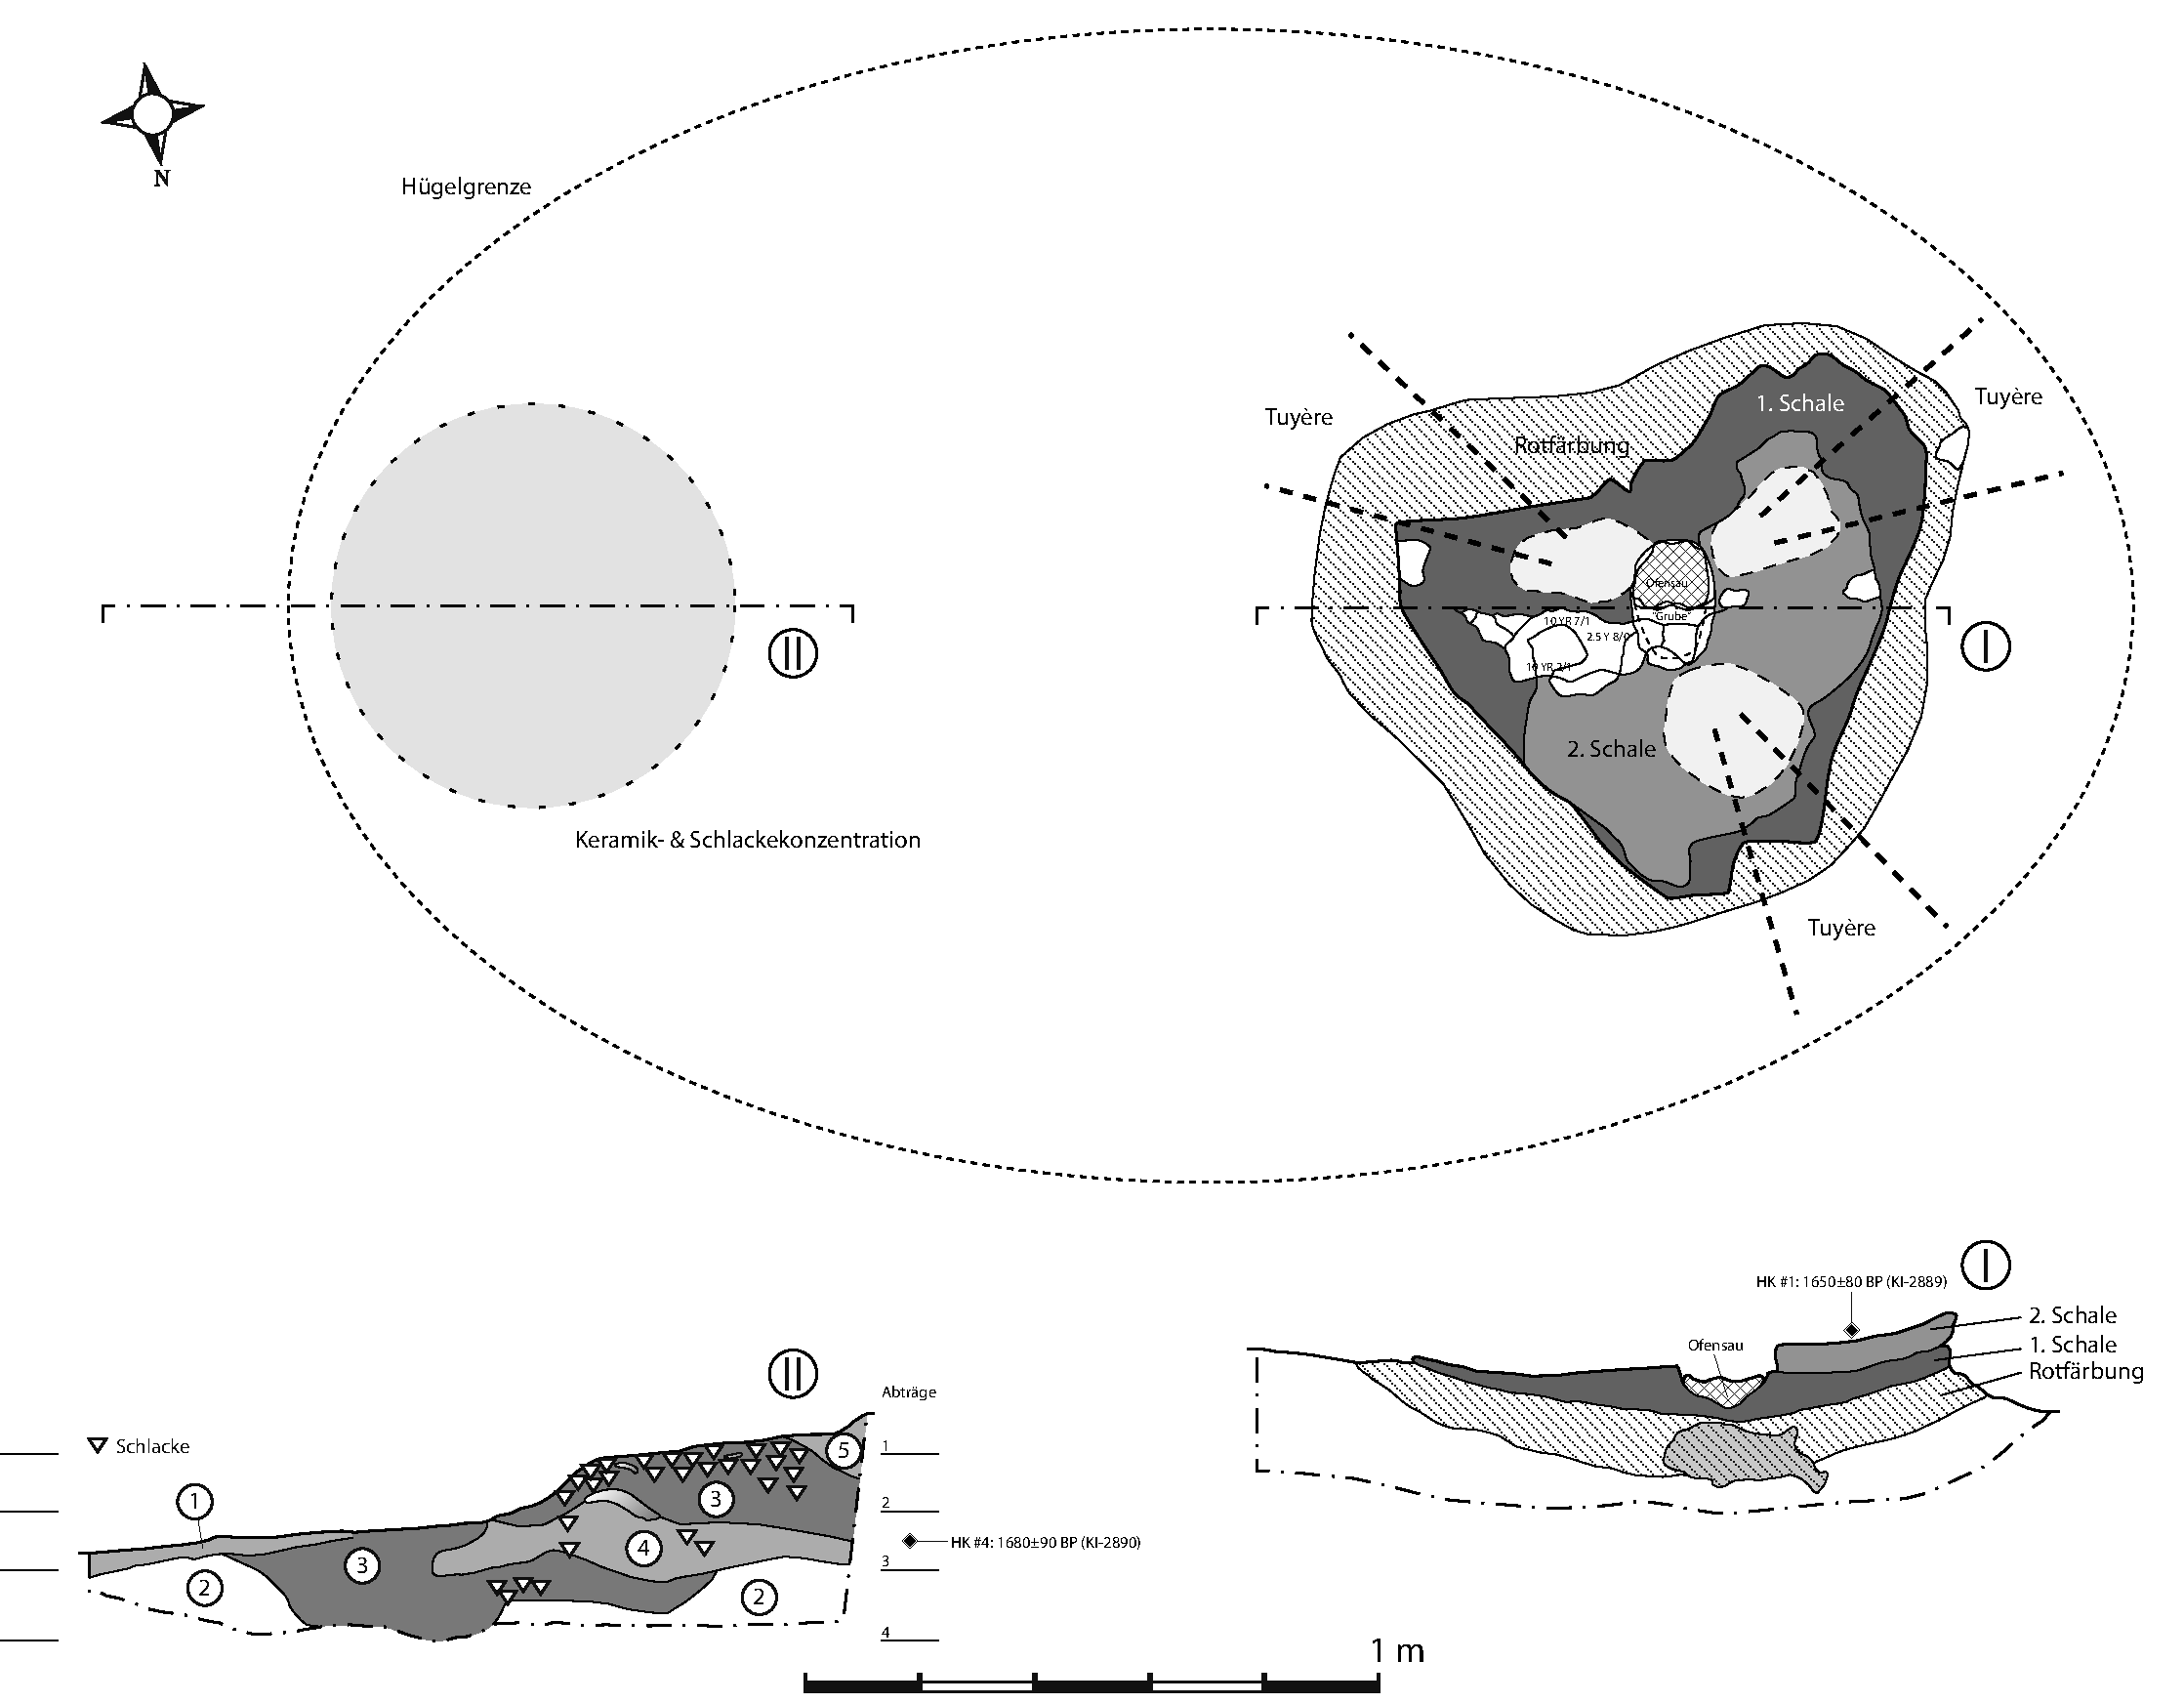
\includegraphics[width=.9\textwidth]{fig/MUN87-3.pdf}
		\caption{MUN~87/3: Planum und Profile.}
		\label{fig:MUN87.3_PlanumProfile}
	\end{subfigure}
	\caption{MUN~87/3: Übersicht über die Ofenplattform und die angelegten Profilschnitte.}
	\label{fig:MUN87.3.I_Planum+ProfilSüd_Foto}
\end{figure*}

\section*{\begin{tabular*}{\linewidth}{@{}l @{\extracolsep{\fill}} r@{}}
		Nr.~18 & MUN~87/3 \\
	\end{tabular*} 
}

\textsf{\textbf{Munda (Likwala-aux-Herbes; Fpl.~304)}}

\vspace{1em}

\noindent\begin{tabular}{@{}rl@{}}
	\textbf{Feldarbeit:} & \textbf{19.08.--24.08.1987 (H. Holsten)} \\ 
	\textbf{Abb.:} & \textbf{\ref{fig:MUN87.3-0_Foto}--\ref{fig:MUN87-3_14C-Kalibration}} \\ 
	\textbf{Tab.:} & \textbf{\ref{tab:MUN87-3_Funde}--\ref{tab:MUN87-3_14C-Daten}}\\
	\textbf{Taf.:} & \textbf{94.1--3} \\ 
	\textbf{Lit.:} & \textbf{--} \\ 
\end{tabular} 

\paragraph{Grabung und Befunde}\hspace{-.5em}|\hspace{.5em}%
Auf einer ovalen, etwa 3\,$\times$\,2\,m großen und 0,3--0,4\,m hohen Erhebung, die sich unmittelbar nördlich einer kleinen Hütte befand (Abb.~\ref{fig:MUN87_Fundstelle}), wurde eine dreieckige, flache Schale aus gebranntem Ton beobachtet (Abb.~\ref{fig:MUN87.3-0_Foto}, \ref{fig:MUN87.3.I_Planum+ProfilSüd_Foto}). Die Plattform lag am westlichen Rand des flachen Hügels und hatte eine Kantenlänge von jeweils etwa 0,9\,m. Am östlichen Rand des Hügels, in Richtung Flussufer, und etwa 1\,m von der Ofenschale entfernt, wurde eine etwa 0,7\,m große Keramik- und Schlacke-Konzentration erfasst. Die beiden Bereiche wurden schließlich getrennt voneinander untersucht: die Lehmplatte wurde unter der Befundnummer MUN~87/3/I und die Schlacke- und Keramikkonzentration unter der Kennung MUN~87/3/II ausgegraben.

Die flache Ofenschale lag auf dem anstehenden gelben Ton auf. Ihr Rand war zum Zeitpunkt der Grabung teilweise erodiert. Bereits nach dem Putzen wurde deutlich, dass den Rand der Schale ein etwa 12--18\,cm breiter Streifen rot verziegelter, anstehender Lehm umgab (Abb.~\ref{fig:MUN87-3_Planum}). Die Verziegelung reichte auch unter die flache Ofenwanne (Abb.~\ref{fig:MUN87-3_Profile}).\footnote{Der rotgebrannte, verziegelte Bereich ist unterhalb der Ofenschalen noch etwa 7--8\,cm mächtig und geht in den anstehenden gelb-grauen Lehm über (Abb.~\ref{fig:MUN87-3_Profile}). Im Zentrum ist die Verzeigelung, wie auch die Tonwanne selbst, am mächtigsten. Unterhalb der Eisenschlacke-Konzentration in der Eintiefung befand sich eine 0,5--1,5\,cm dicke Schicht ungebrannten grau-braunen Tones. Erst unterhalb dieser trat das rotverziegelte Anstehende zu Tage.} Auch dass die Ofenplatte aus zwei übereinander liegenden Lehmschalen besteht, konnte bereits nach dem ersten Putzen der Oberfläche erkannt werden (Abb.~\ref{fig:MUN87.3_PlanumProfile}. \ref{fig:MUN87-3_Profile}).\footnote{Durch einen ersten, kleinen Profilschnitt wurde die nördliche Hälfte der Ofenplatte abgenommen. Darin konnte die Lehmplatte sowie die rote Verziegelung darunter erfasst werden. Im Anschluss wurde der gesamte nördliche Teil der Ofenplatte entfernt und ein etwa Ost--West-orientiertes Profil angelegt (Abb.~\ref{fig:MUN87.3_PlanumProfile} I).} Die obere, zweite Schale war bereits stark erodiert. Sie besteht aus einem schwarz gebrannten Ton und war noch 3--5\,cm mächtig. Die direkt darunter liegende Schale bestand aus dem gleichen Material und war noch etwa 5\,cm mächtig. Im Zentrum befand sich eine kleine grubenartige, etwa 16\,$\times$23\,cm große Vertiefung. In ihrer südlichen Hälfte enthielt diese einen 5--6\,cm dicken Eisenschlacke-Brocken. An drei Stellen war die Oberfläche beider Ofenschalen nicht dunkelgrau bis schwarz, sondern hellgrau bis weiß.\footnote{Dieses Zeichen einer höheren Hitzeentwicklung kann als Indiz für die Anordnung von drei Tuyères zur Belüftung des Verhüttungsprozesses gedeutet werden.} Die drei auffällig hellen Zonen weisen jeweils in die Ecken der Plattform.

Anders als bei den anderen, in Munda untersuchten Verhüttungsbefunden (Kat.-Nr.~15--16), wurden durch die Grabung MUN~87/3 keine Fragmente von Ofenwandung erfasst. Dies legt nahe, dass der Befund keinen aufgehenden Ofenschacht aufwies und es sich um einen offenen, flachen Schalenofen handelt. Zwischen der Ofenplattform (MUN~87/3/I) und der Keramik-Schlacken-Konzentration (MUN~87/3/II) war weder im Profil noch Planum eine durch Funde oder eine Verfärbung gekennzeichnete, funktionale Verbindung erkennbar.\footnote{Um sicher zu gehen, wurde der stehengebliebene südliche Teil der Plattform am Ende der Grabung abgebrochen und ein grobes Planum angelegt. Dieses erbrachte keine Hinweise auf weitere Eingrabungen oder einen Schlackenausflusskanal.}

In der etwa 1\,m östlich der Plattform (MUN~87/3/I) gelegenen Keramik- und Schlackekonzentration war die Gefäßkeramik wie auch die Schlacken zum Teil sehr stark durch ein lateritähnliches \textit{Bindemittel} miteinander verklebt und eine Bergung nur schwer möglich (Abb.\ref{fig:MUN87.3.II-3_Foto}). Die Keramik ist sehr fragil und ihre Oberfläche meist stark angelöst. Es konnte auch keine klare Begrenzung der Keramik-Schlacken-Konzentration erfasst werden. Lediglich durch die maximale Fundstreuung konnte die Ausdehnung der Struktur eingegrenzt werden (Abb.~\ref{fig:MUN87.3_PlanumProfile}).\footnote{Im Anschluss an die Dokumentation des Profils wurden beim Abtragen der südlichen Hälfte eine Vielzahl von Tuyère-Fragmenten und Schlacken sowie bis zu 15\,cm große, gebrannte Tonbrocken gefunden.}

\vspace{1.5em}
\noindent Das Profil durch die Keramik-Schlacken-Kon"-zen"-tra"-tion (MUN~87/3/II) zeigte die folgende Abfolge von Schichten (Abb.~\ref{fig:MUN87.3.II-3_Foto}, \ref{fig:MUN87.3_PlanumProfile}):
\begin{itemize}[leftmargin=*, labelindent=1em, noitemsep, topsep=0pt]
\item [(1)] 10YR 4/4; fein gebänderte, regendurchweichte \textit{Schlämmschicht}
\item [(2)] 7.5YR 6/8; rötlich-gelber, von grauen Gängen durchzogener, anstehender Ton
\item [(3)] 10YR 3/3; dunkelgrauer, mit Keramik und Schlacke und Holzkohle durchsetzter Lehm
\item [(4)] k.a.
\item [(5)] 10YR 6/6 bis 10YR 5/3; gelb-grauer durchmischter Lehm
\end{itemize}

\paragraph{Keramik\vspace{.5em}}\mbox{}\\
\begin{tabular}{@{}lrl@{}}
Ausgezählt: & 441\,g & \\ 
Bearbeitet: & 1796\,g & (80\,\%) \\ 
Insgesamt: & 2237\,g & \\ 
\end{tabular} 

\begin{table*}[p]
\centering
{\footnotesize\begin{sftabular}{@{}lrrrr@{}}
\toprule
\textbf{Fundkategorie} &  \textbf{Anzahl} &    \textbf{\%} &  \textbf{Gewicht (kg)} &    \textbf{\%} \\
\midrule
     Schlacke &     195 &  65,7 &         10,35 &  76,5 \\
      Keramik &      55 &  18,5 &          2,24 &  16,5 \\
       Tuyère &      38 &  12,8 &          0,91 &   6,7 \\
     Ofenwand &       7 &   2,4 &          0,00 &   0,0 \\
        Stein &       1 &   0,3 &          0,02 &   0,2 \\
     Sonstige &       1 &   0,3 &          0,00 &   0,0 \\
\bottomrule
\end{sftabular}
}
\caption{MUN~87/3: Anteil verschiedener Fundmaterialien.}
\label{tab:MUN87-3_Funde}
\end{table*}

\begin{figure*}[p]
	\centering
	\begin{subfigure}[t]{0.3\textwidth}
		\centering
		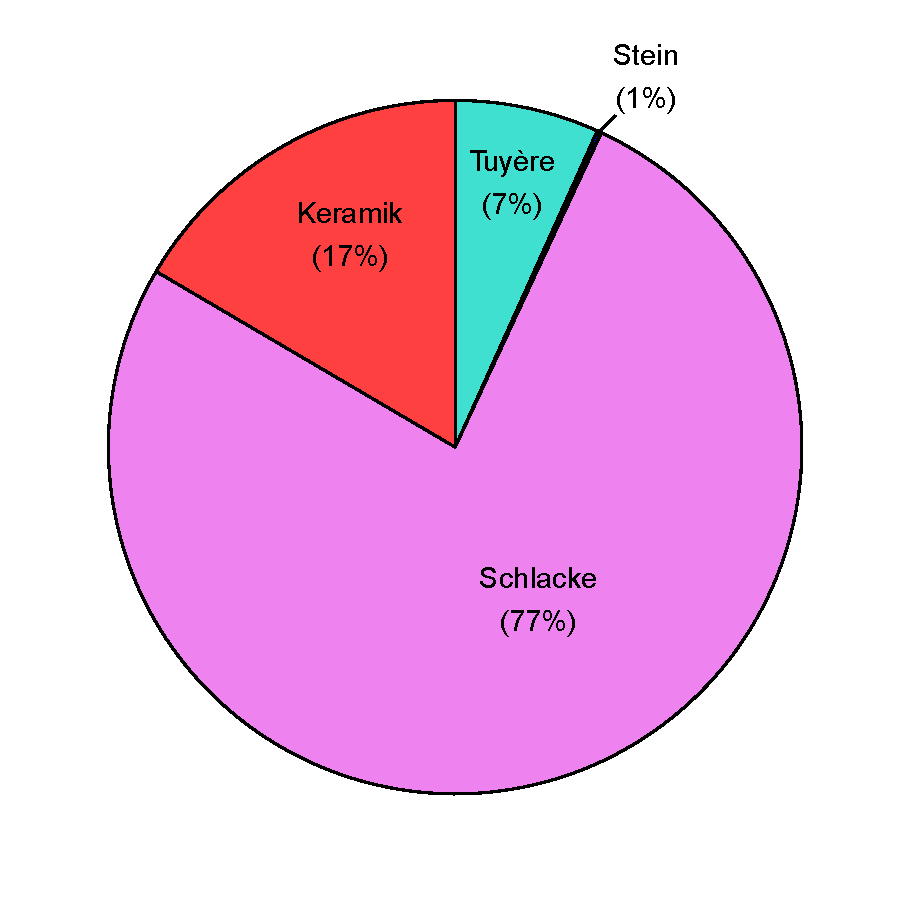
\includegraphics[width = \textwidth]{fig/9-18_MUN87-3_Funde_R_modDS.pdf}
		\caption{Funde}
		\label{fig:MUNPIK87-3_FundeArt}
	\end{subfigure}\hfill
	\begin{subfigure}[t]{0.3\textwidth}
		\centering
		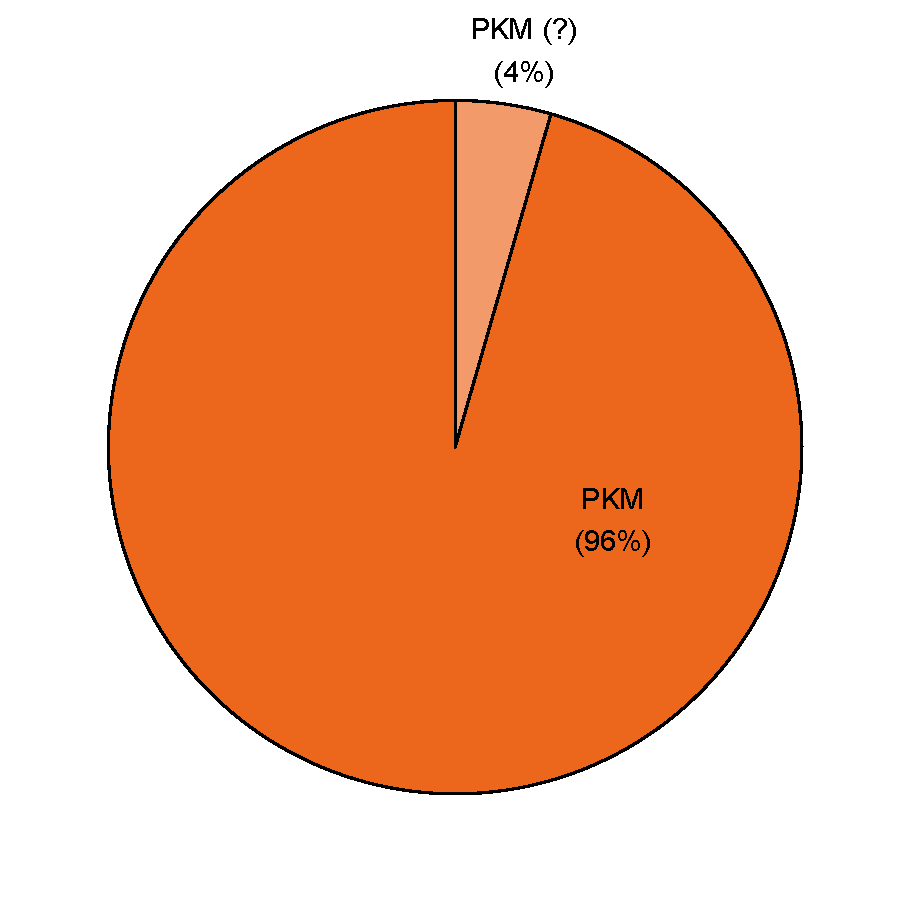
\includegraphics[width = \textwidth]{fig/9-18_MUN87-3_Stilgruppen_R_modDS.pdf}
		\caption{keramische Stilgruppen}
		\label{fig:MUN87-3_Stilgruppen}
	\end{subfigure}\hfill
	\begin{subfigure}[t]{0.3\textwidth}
		\centering
		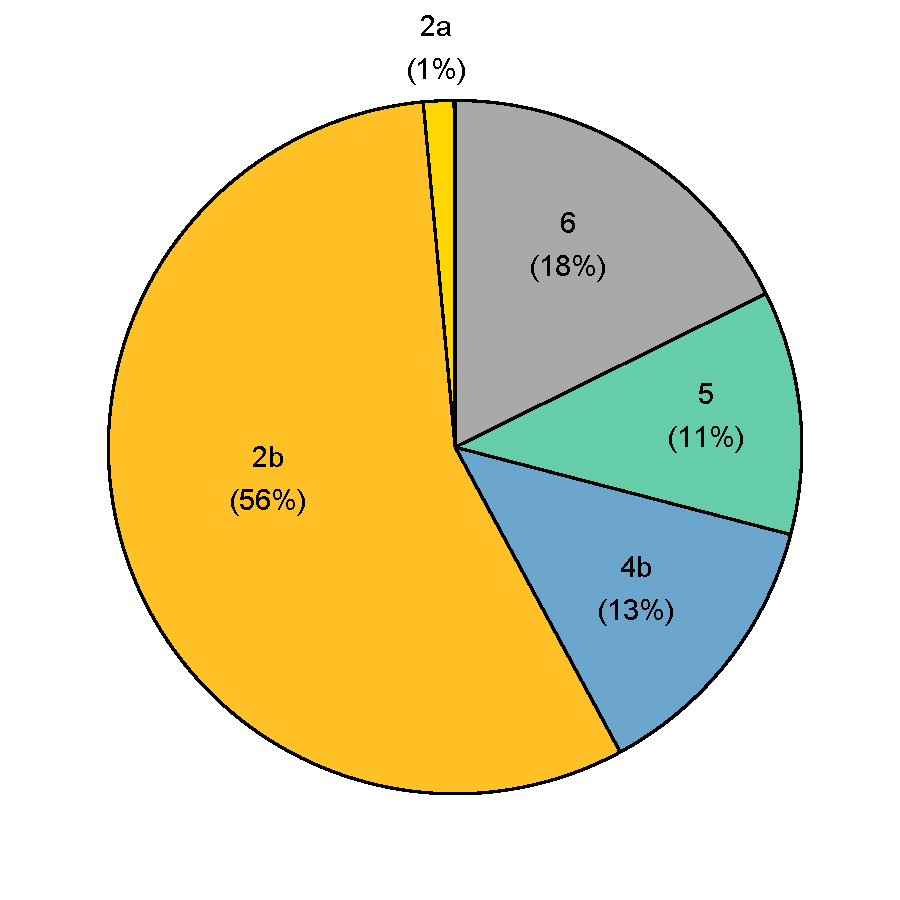
\includegraphics[width = \textwidth]{fig/9-18_MUN87-3_Schlacketypen_R_modDS.pdf}
		\caption{Schlacketypen\vspace{1em}}
		\label{fig:MUN87-3_SchlackeTyp}
	\end{subfigure}
	\begin{subfigure}[t]{\textwidth}
		\centering
		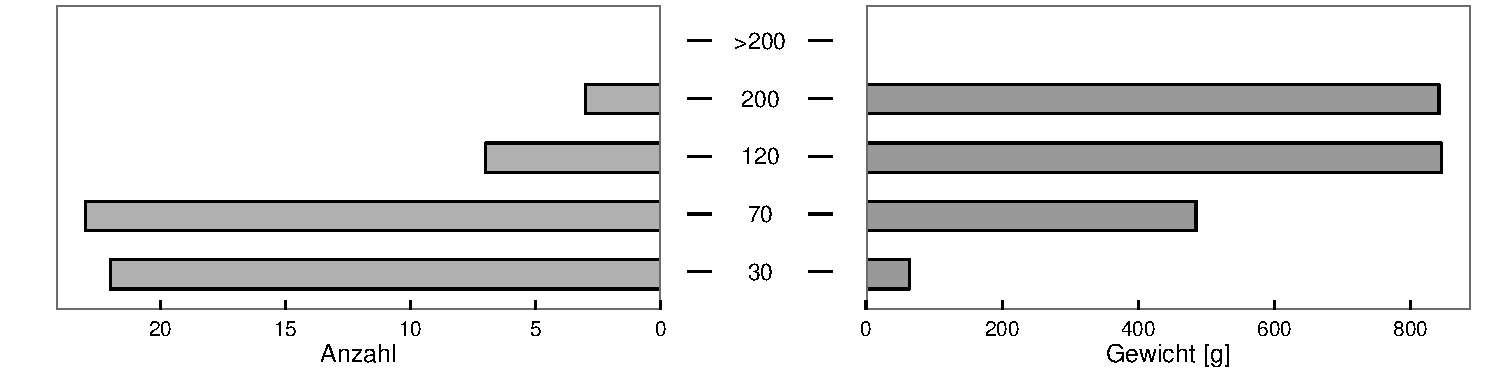
\includegraphics[width = \textwidth]{fig/9-15_MUN87-3_Fragmentierung_2.pdf}
		\caption{Fragmentierung}
		\label{fig:MUN87-3_Fragmentierung}
	\end{subfigure}
	\caption{MUN~87/3: Anteile der Fundmaterialien (A), keramischen Stilgruppen (B) und Schlacken (C) sowie Fragmentierungsgrad der Scherben (n~=~55; Größenklassen siehe Anm.~\ref{ftn:Keramik_Fragmentierung}).}
	\label{fig:MUN87-3_Funde}
\end{figure*}

\begin{figure*}[p]
	\begin{minipage}{\textwidth}
		\centering
		{\footnotesize\begin{sftabular}{@{}llllll@{}}
			\toprule
			\textbf{Lab-Nr} & \textbf{Datum (bp)} & \textbf{Datum (2-Sigma)} & \textbf{Befundteil} & \textbf{Abtrag} & \textbf{Tiefe (unter NP)} \\ 
			\midrule
			KI-2889 & 1650~\( \pm \)~80 & 218--593 n.~Chr. & I & Oberfläche 2. Schale (HK 1) & 0\,m \\ 
			KI-2890 & 1680~\( \pm \)~90 & 134--554 n.~Chr. & II & 3 (HK 4) & 0,50\,m \\ 
			\bottomrule 
		\end{sftabular}}
		\captionof{table}{MUN~87/3: Radiokohlenstoffdatierungen.}
		\label{tab:MUN87-3_14C-Daten}
	\end{minipage}
	
	\vspace{2em}
	
	\begin{minipage}{\textwidth}
		\centering
		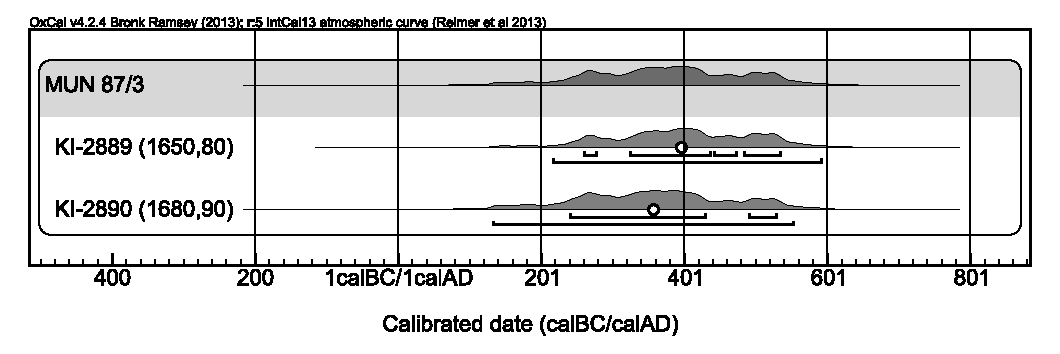
\includegraphics[width = .75\textwidth]{fig/MUN87_3_14C.pdf}
		\captionof{figure}{MUN~87/3: Kalibrierung der Radiokohlenstoffdatierungen aus den beiden Befundteilen I \& II.}
		\label{fig:MUN87-3_14C-Kalibration}
	\end{minipage}
\end{figure*}

\vspace{1em}
\noindent Das Fundinventar aus den beiden Profilschnitten umfasst etwa 10\,kg Schlacken (Tab.~\ref{tab:MUN87-3_Funde}).\footnote{Nur etwa 40\,\% dieser Schlacken wurden ausgeführt und stehen für weitere Untersuchungen zur Verfügung. Lediglich 3\,\% der insgesamt gefundenen Schlacken stammen aus dem Bereich der Ofenwanne.} In der Keramik-Schlacke-Konzentration wurden etwa 2\,kg Keramik ausgegraben. 

Die Erhaltung der Keramik ist im Allgemeinen sehr schlecht. Alle Stücke sind aus weißbrennenden Tonen und ohne den Zusatz nichtplastischer Partikel hergestellt. Die Hälfte aller Stücke lässt sich dem nur eine schwache randliche Oxidation aufweisenden \textit{Fabric} 1a zurechnen. Grundsätzlich zeigt das keramischen Inventar aus der Grabung MUN~87/3 starke Parallelen zu dem Inventar aus dem oberen Verfüllungsbereich C der Gruben MUN~87/2-1-1 (Kat.-Nr.~16; Taf.~91.1--5). Es umfasste keine Formen, die nicht dem Pikunda-Munda-Stil (Kap.~\ref{sec:PKM-Gr}) zugewiesen werden können (Abb.~\ref{fig:MUN87-3_Stilgruppen}). Die durchweg rundbodige Keramik umfasst Fragmente einiger Pikunda-Munda-Schalen des Typs F3 mit geraden oder nur leicht konkaven Gefäßwandungen und charakteristisch scharfem Knick zwischen Wandung und Boden (Taf.~94.1). Die Scherben sind mittels Wiegebandmustern (Tab.~\ref{tab:Verzierungselemente}: 04.2) und horizontalen Rillen (Tab.~\ref{tab:Verzierungselemente}: 02.1) oder Winkelmustern (Tab.~\ref{tab:Verzierungselemente}: 01.6) verziert.

\paragraph{Sonstige Funde}\hspace{-.5em}|\hspace{.5em}%
Den größten Anteil am Fundmaterial aus MUN~87/3 machen etwa 10\,kg Schlacken aus, von denen etwa 40\,\% exportiert wurden und aufgenommen werden konnten.\footnote{Obschon es sich um eine repräsentative Auswahl handelte, sind alle folgenden Ausführungen über die Anteile und Verteilung der Schlacken mit Vorbehalten zu versehen. Über die Hälfte aller Schlacken sind kleiner als 30\,$\times$\,30\,mm, während weitere 40\,\% kleiner als 70\,$\times$\,70\,mm sind. Größere Stücke kommen nur sehr selten vor.} Das Inventar setzt sich vor allem aus grünlichen Fließschlacken hoher Viskosität vom Typ~2b zusammen (Abb.~\ref{fig:MUN87-3_SchlackeTyp}). Zusammen mit einigen wenigen Schlacken des Typs~2a machen diese insgesamt 60\,\% aller aufgenommenen Schlacken aus. Die kantigen Schlacken geringer Viskosität des Typs~4 sind mit etwa 14\,\% deutlich seltener vertreten, während die ansonsten in Munda kaum beobachtete Schlackenbreccie des Typs~5 mit einem Anteil von 8\,\% erstaunlich deutlich vertreten ist.\footnote{Ähnlich häufig wurde dieser Typ Schlacke lediglich in der jüngeren Grube A im Schnitt PIK~87/1 in Pikunda am \mbox{Sangha} beobachtet (Kat.-Nr.~8).} potenzielle Schmiedeschlacke des Typs~6 sind mit 18\,\% ebenfalls auffällig häufig belegt.\footnote{Ähnlich hohe Anteile potenzieller Schmiedeschlacken fanden sich nur in der oberen Verfüllung C der in der Grabung MUN~87/2-1-1 erfassten Grube (Kat.-Nr.~16).}

\paragraph{Datierung}\hspace{-.5em}|\hspace{.5em}%
Aus dem Befund liegen zwei, fast gleich alte Radiokohlenstoffdatierungen vor, die den Befund in das 3.--6.~Jh. n.~Chr. datieren (Tab.~\ref{tab:MUN87-3_14C-Daten}, Abb.~\ref{fig:MUN87-3_14C-Kalibration}). Während eine der beiden datierten Proben aus dem Bereich der Ofenplatte stammt (KI-2889), wurde die zweite in der Keramik-Schlacke-Konzentration genommen (KI-2890). Durch die sich stark überlappenden Datierungen kann ein Zusammenhang zwischen der Ofenplatte und der Keramik-Schlacke-Konzentration als wahrscheinlich angenommen werden. 

\paragraph{Interpretation}\hspace{-.5em}|\hspace{.5em}%
Durch die Grabung MUN~87/3 wurde ein offener Ofen beziehungsweise potenzielle Schmiedeesse erfasst, die sich auf einem kleinen, flachen Hügel befand und in das 3.--6.~Jh. n.~Chr. datiert werden kann. Es handelt sich um den jüngsten Komplex, in dem Keramik des Pikunda-Munda-Stils erfasst wurde. Der Befund zeichnet sich, ähnlich wie die offenen Öfen vom Typ \textit{Bamanya} \parencite[3235--3237]{Eggert.1987}, durch eine flache Lehmplattform aus, die keine aufgehenden Elemente beziehungsweise Ofenwand aufweist. Im Fall des Befundes aus MUN~87/3 erfolgte die Belüftung wohl mittels drei sternförmig angeordneter Tuyères, deren Lage durch weiß-gebrannte Bereiche auf der Lehmplatte angezeigt sind. Der aus zwei übereinander liegenden Schalen bestehende Befund legt nahe, dass die Einrichtung mehrfach genutzt und erneuert wurde. Da sich die Ausrichtung der weißgebrannten, mutmaßlich die Position von Tuyères anzeigenden Stellen zwischen den beiden Schalen nicht unterscheidet, kann von einem zeitlich engen Zusammenhang dieser beiden Nutzungsphasen ausgegangen werden. Im Unterschied zu den offenen Öfen des Typs \textit{Bamanya} weist der Befund MUN~87/3 jedoch keine seitliche Schlackenausflussgrube auf. Auch umfassen die Schlacken einen auffällig hohen Anteil potenzieller Schmiedeschlacken.